% !TEX encoding = UTF-8
% !TEX TS-program = pdflatex
% !TEX root = ../tesi.tex

%**************************************************************
\chapter{Messages}
\label{cap:messages}
%**************************************************************

%**************************************************************
\section{Structure of packets}

There is one generic packet that will be exchanged during the client - server communication. It is made of: \newline{}
\begin{itemize}
	\item AAD (24 bytes)
	\item IV (12 bytes)
	\item PAYLOAD (variable size defined inside the AAD)
	\item TAG (16 bytes)
\end{itemize}
The AAD content is represented in the Table \ref{tab:AAD-content}.
\begin{longtable}{|p{0.4\textwidth}|p{0.2\textwidth}|}
	\caption{AAD content}
	\label{AAD content} 
	\label{tab:AAD-content} \\
	\hline
	\textbf{Content} & \textbf{Size} \\
	\hline
	Operation ID & 4 bytes \\
	\hline
	Message counter & 8 bytes \\
	\hline
	Payload length & 8 bytes \\
	\hline
	Number of Packets & 4 bytes \\
	\hline
\end{longtable}%

An in depth description of every single content of the AAD is necessary:

\begin{itemize}
	\item \textbf{Operation ID}: represents an integer number that will indicate the type of the operation to be done. The values that Operation ID can have will be listed at \ref{tab:operation-ids-list};
	\item \textbf{Message counter}: counter of the number of messages exchanged between server and client, it is used to avoid replay attack and as such must be in sync both client side and server side;
	\item \textbf{Payload length}: the payload length will be variable and this data will be used to know how many bytes to expect as payload;
	\item \textbf{Number of packets}: Some operations will send data in multiple packets, this value is used to know how many packets to expect.
\end{itemize}

\begin{longtable}{|p{0.06\textwidth}|p{0.15\textwidth}|p{0.79\textwidth}|}
	\caption{Operation ID values and description}
	\label{Operation ID list} 
	\label{tab:operation-ids-list} \\
	\hline
	\textbf{Value} & \textbf{Operation} & \textbf{Description} \\
	\hline
	 0 & ACK & Message received, the operation is allowed and can continue \\
	\hline
	 1 & UPLOAD & Client operation used to ask the server for permission to upload a local file to remote \\
	\hline
	 2 & DOWNLOAD & Client operation used to ask the server for permission to download a remote file to local \\
	\hline
	 3 & DELETE & Client operation used to ask the server for permission to delete a remote file \\
	\hline
	 4 & LIST & Client operation used to ask the server the list of remote files  \\
	\hline
	 5 & RENAME & Client operation used to ask the server to rename a remote file \\
	\hline
	 6 & LOGOUT & Client operation used to gracefully close the connection \\
	\hline
	 7 & DONE & Used to communicate that the previous operation has been completed successfully \\
	\hline
	 8 & ABORT & Message received, the operation is not allowed and cannot continue \\
	\hline
	 9 & DATA & The packet contains file data \\
	\hline
\end{longtable}%

\section{Operations}

In this section every operation and its sequence diagram will be discussed and explained.

\subsection{Upload}

\begin{figure}[!h] 
    \centering 
    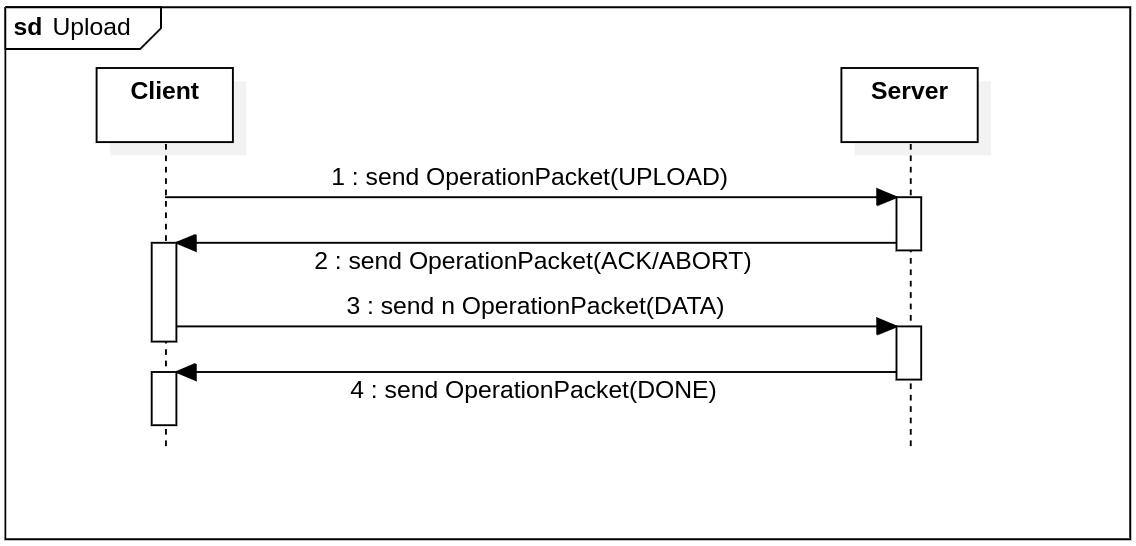
\includegraphics[width=1\columnwidth]{chapter-3/Upload.png} 
    \caption{Upload operation.}
    \label{fig:upload_operation}
\end{figure}

\subsection{Download}

\begin{figure}[!h] 
    \centering 
    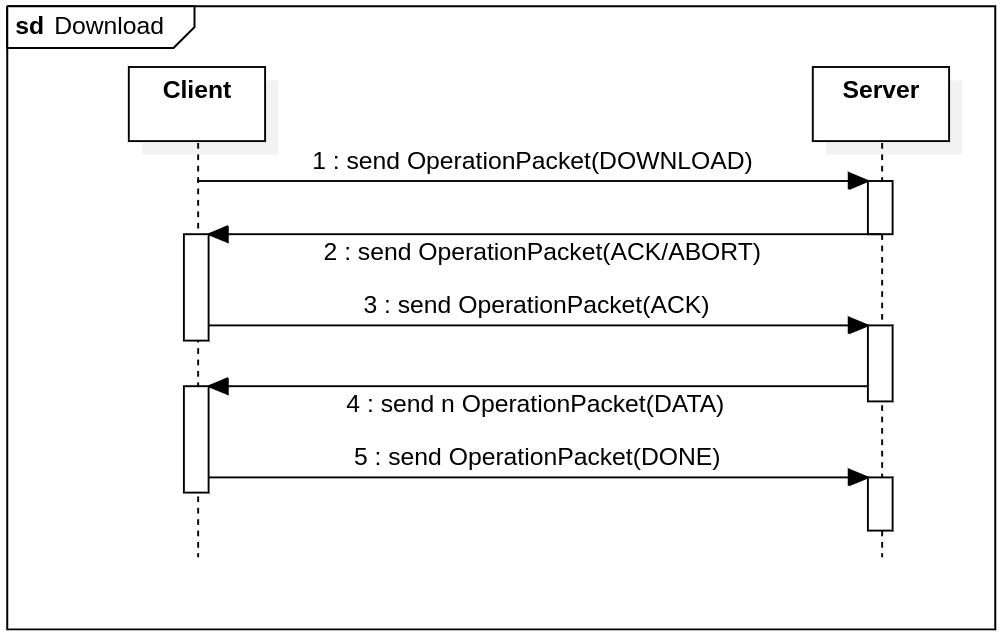
\includegraphics[width=1\columnwidth]{chapter-3/Download.png} 
    \caption{Download operation.}
    \label{fig:download_operation}
\end{figure}

\subsection{List}

\begin{figure}[!h] 
    \centering 
    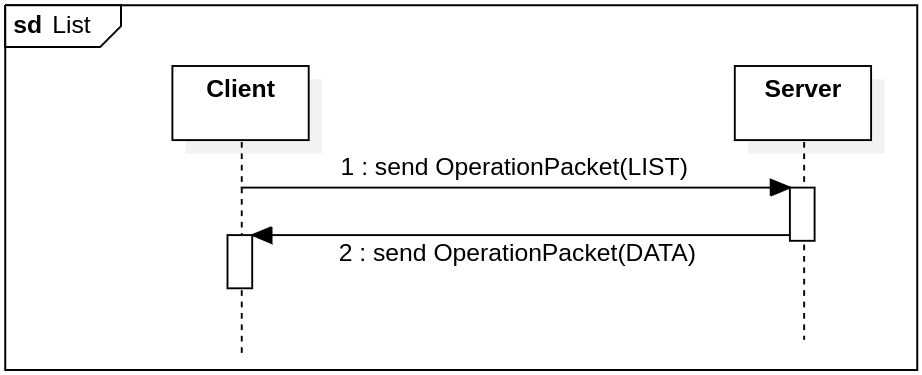
\includegraphics[width=1\columnwidth]{chapter-3/List.png} 
    \caption{List operation.}
    \label{fig:list_operation}
\end{figure}

\subsection{Delete}

\begin{figure}[!h] 
    \centering 
    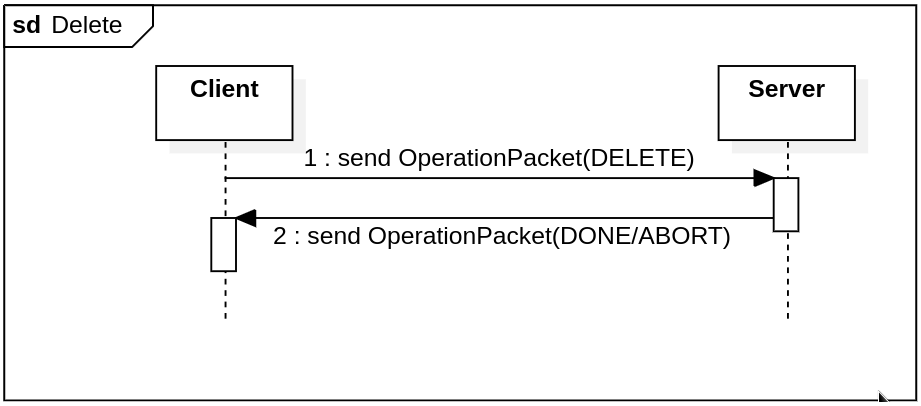
\includegraphics[width=1\columnwidth]{chapter-3/Delete.png} 
    \caption{Delete operation.}
    \label{fig:delete_operation}
\end{figure}

\subsection{Rename}

\begin{figure}[!h] 
    \centering 
    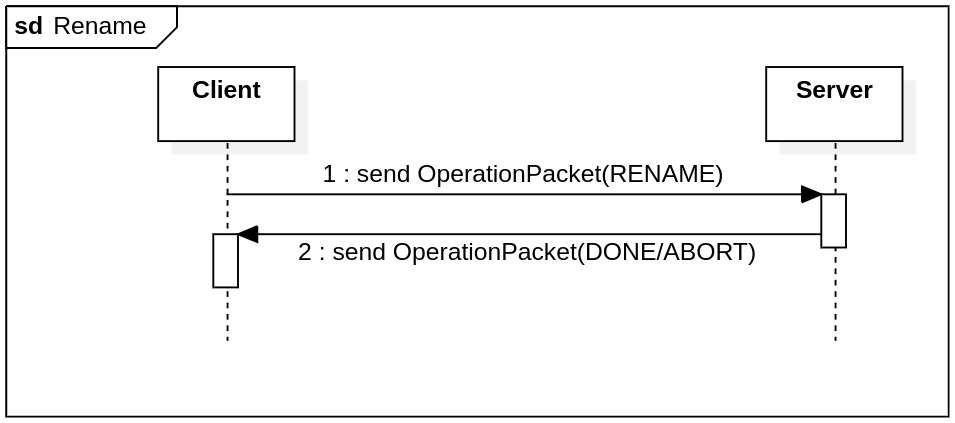
\includegraphics[width=1\columnwidth]{chapter-3/Rename.png} 
    \caption{Rename operation.}
    \label{fig:rename_operation}
\end{figure}

\subsection{Logout}

\begin{figure}[!h] 
    \centering 
    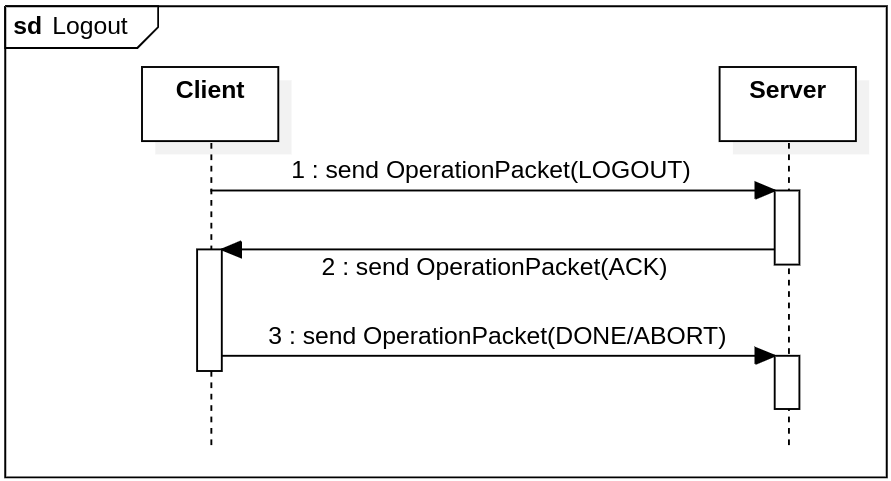
\includegraphics[width=1\columnwidth]{chapter-3/Logout.png} 
    \caption{Logout operation.}
    \label{fig:logout_operation}
\end{figure}
